
\chapter{Essay: Software engineers and software artisans}

Let us look at the differences between the kind of activities we ordinarily
call engineering, as opposed to artisanship or craftsmanship. It will
then become apparent that today's computer programmers are better
understood as ``software artisans'' rather than software engineers.

\section{Engineering disciplines }

Consider what kinds of process a mechanical engineer, a chemical engineer,
or an electrical engineer follows in their work, and what kind of
studies they require for proficiency in their work.

A mechanical engineer \href{https://www.colorado.edu/mechanical/undergraduate-students/curriculum}{studies}
calculus, linear algebra, differential geometry, and several areas
of physics such as theoretical mechanics, thermodynamics, and elasticity
theory, and then uses calculations to guide the design of a bridge,
say. A chemical engineer \href{https://www.colorado.edu/engineering/sample-undergraduate-curriculum-chemical}{studies}
chemistry, thermodynamics, calculus, linear algebra, differential
equations, some areas of physics such as thermodynamics and kinetic
theory, and uses calculations to guide the design of a chemical process,
say. An electrical engineer \href{https://seas.yale.edu/departments/electrical-engineering/undergraduate-study/undergraduate-curriculum-information}{studies}
advanced calculus, linear algebra, as well as several areas of physics
such as electrodynamics and quantum physics, and uses calculations
to guide the design of an antenna or a microchip.

The pattern here is that an engineer uses mathematics and natural
sciences in order to design new devices. Mathematical calculations
and scientific reasoning are required \emph{before} drawing a design,
let alone building a real device or machine.

Some of the studies required for engineers include arcane abstract
concepts such as a ``\href{https://serc.carleton.edu/NAGTWorkshops/mineralogy/mineral_physics/tensors.html}{rank-4 elasticity tensor}''
(used in calculations of elasticity of materials), ``\href{https://arxiv.org/abs/math/0008147}{Lagrangian with non-holonomic constraints}''
(used in robotics), the ``Gibbs free energy'' (for \href{https://www.amazon.com/Introduction-Chemical-Engineering-Kinetics-Reactor/dp/1118368258}{chemical reactor design}),
or the ``\href{https://www.youtube.com/watch?v=KAbqISZ6SHQ}{Fourier transform of the delta function}''
and the ``\href{https://ocw.mit.edu/resources/res-6-008-digital-signal-processing-spring-2011/video-lectures/lecture-6-the-inverse-z-transform/}{inverse Z-transform}''
(for digital signal processing).

To be sure, a significant part of what engineers do is not covered
by any theory: the \emph{know-how}, the informal reasoning, the traditional
knowledge passed on from expert to novice,  \textendash{}  all those
skills that are hard to formalize. Nevertheless, engineering is crucially
based on natural science and mathematics for some of its decision-making
about new designs.

\section{Artisanship: Trades and crafts }

Now consider what kinds of things shoemakers, plumbers, or home painters
do, and what they have to learn in order to become proficient in their
profession.

A novice shoemaker, for example, would begin by \href{https://youtu.be/cY5MY0czMAk?t=141}{copying some drawings}
and then cutting leather in a home workshop. Apprenticeships proceed
via learning by doing while listening to comments and instructions
from an expert. After a few years of apprenticeship (for example,
a \href{http://www.calapprenticeship.org/programs/painter_apprenticeship.php}{painter apprenticeship in California}
can be as short as 2 years), a new specialist is ready to start productive
work. 

All these trades operate entirely from tradition and practical experience.
The trades do not require any academic study because there is no formal
theory from which to proceed. To be sure, there is \emph{a lot} to
learn in the crafts, and it takes a large amount of effort to become
a good artisan in any profession. But there are no rank-4 tensors
to calculate, nor any differential equations to solve; no Fourier
transforms to apply to delta functions, and no Lagrangians to check
for non-holonomic constraints.

Artisans do not study any formal science or mathematics because their
professions do not make use of any \emph{formal computation} for guiding
their designs or processes.

\section{Programmers today are artisans, not engineers }

Now I will argue that programmers are \emph{not engineers} in the
sense we normally see the engineering professions.

\subsection{No requirement of formal study }

According to this recent Stack Overflow survey, \href{https://thenextweb.com/insider/2016/04/23/dont-need-go-college-anymore-programmer/}{about half of the programmers do not have a degree in Computer Science}.
I am one myself; my degrees are in physics, and I have never formally
studied computer science. I took no academic courses in algorithms,
data structures, computer networks, compilers, programming languages,
or any other topics ordinarily included in the academic study of ``computer
science''. None of the courses I took at university or at graduate
school were geared towards programming. I am a completely self-taught
software developer.

There is a large number of successful programmers who \emph{never}
studied at a college, or perhaps never studied formally in any sense.
They acquired all their knowledge and skills through self-study and
practical work. \href{https://en.wikipedia.org/wiki/Robert_C._Martin}{Robert C. Martin}
is one such prominent example; an outspoken guru in the arts of programming
who has seen it all, he routinely \href{https://blog.cleancoder.com/uncle-bob/2013/02/01/The-Humble-Craftsman.html}{refers to programmers as artisans}
and uses the appropriate imagery: novices, trade and craft, the ``honor
of the guild'', etc. He compares programmers to plumbers, electricians,
lawyers, and surgeons, but not to mathematicians, physicists, or engineers
of any kind. According to \href{https://blog.cleancoder.com/uncle-bob/2013/11/25/Novices-Coda.html}{one of his blog posts},
he started working at age 17 as a self-taught programmer, and then
went on to more jobs in the software industry; he never mentions going
to college. It is clear that R.~C.~Martin \emph{is} an expert craftsman,
and that he did not need academic study to master his craft.

Here is \href{https://www.quora.com/Can-you-become-a-software-engineer-without-actually-going-to-university-college-How}{another opinion}
(emphasis is theirs):
\begin{quotation}
Software Engineering is unique among the STEM careers in that it absolutely
does \emph{not} require a college degree to be successful. It most
certainly does not require licensing or certification. \emph{It requires
experience}.
\end{quotation}
This is a description that fits a career in crafts \textendash{} but
certainly not a career, say, in electrical engineering.

The high demand for software developers gave rise to ``\href{https://cvbj.biz/2018/03/15/demand-software-developers-continues-soar-heres-cheapest-free-way-start-tech-career/}{developer boot camps}''
\textendash{} vocational schools that prepare new programmers very
quickly, with no formal theory or mathematics involved, through purely
practical training. These vocational schools \href{https://www.fullstackacademy.com/blog/why-are-some-coding-bootcamps-job-placement-rates-so-high}{are successful}
in job placement. But it is unimaginable that a 6-month crash course
or even a 2-year vocational school could prepare an engineer to work
successfully on designing, say, \href{https://www.dwavesys.com/quantum-computing}{quantum computers},
without ever having studied quantum physics or calculus.

\subsection{No mathematical formalism guides software development}

Most books on software engineering contain no formulas or equations,
no mathematical derivations of any results, and no precise definitions
of the various technical terms they are using (such as ``object-oriented''
or ``software architecture''). Some books on software engineering
even have no program code in them \textendash{} just words and illustrative
diagrams. These books talk about how programmers should approach their
job, how to organize the work flow and the code architecture, in vague
and general terms: ``code is about detail'', ``you must never abandon
the big picture'', ``you should avoid tight coupling in your modules'',
``a class must serve a single responsibility'', and so on. Practitioners
such as R.\ C.\ Martin never studied any formalisms and do not think
in terms of formalisms; instead they think in \href{https://blog.cleancoder.com/uncle-bob/2016/03/19/GivingUpOnTDD.html}{vaguely formulated, heuristic \textquotedblleft principles\textquotedblright}.

In contrast, every textbook on mechanical engineering or electrical
engineering has a significant amount of mathematics in it. The design
of a microwave antenna \href{https://www.youtube.com/watch?v=46SbGxS73dY}{is guided}
not by the principle of ``serving a single responsibility'' but
by calculations of wave propagation, based on theoretical electrodynamics.

Donald Knuth's classic textbook is called ``\emph{The Art of Programming}''.
It is full of tips and tricks about how to program; but it does not
provide any formal theory that could guide programmers while actually
\emph{writing} programs. There is nothing in that book that would
be similar to the way mathematical formalism guides designs in electrical
or mechanical engineering. If Knuth's books were based on such formalism,
they would have looked quite differently: some theory would be first
explained and then applied to help us write code.

Knuth's books provide many algorithms, including mathematical ones.
But algorithms are similar to patented inventions: They can be used
immediately without further study. Understanding an algorithm is not
similar to understanding a mathematical theory. Knowing one algorithm
does not make it easier to develop another algorithm in an unrelated
domain. In comparison, knowing how to solve differential equations
will be applicable to thousands of different areas of science and
engineering.

A book exists with the title ``\href{https://www.amazon.com/Science-Programming-Monographs-Computer/dp/0387964800}{Science of Programming}'',
but the title is misleading. The author does not propose a science,
similar to physics, at the foundation of the process of designing
programs, similarly to how calculations in quantum physics predict
the properties of a quantum device. The book claims to give precise
methods that guide programmers in writing code, but the scope of proposed
methods is narrow: the design of simple algorithms for iterative manipulation
of data. The procedure suggested in that book is far from a formal
mathematical \emph{derivation} of programs from specification. (\href{https://www.amazon.com/Program-Derivation-Development-Specifications-International/dp/0201416247}{A book with that title}
also exists, and similarly disappoints.) Programmers today are mostly
oblivious to these books and do not use the methods explained there.

Standard computer science courses today do not teach a true \emph{engineering}
aproach to software construction. They do teach analysis of programs
using formal mathematical methods; the main such methods are \href{https://www.cs.cmu.edu/~adamchik/15-121/lectures/Algorithmic\%20Complexity/complexity.html}{complexity analysis}
(the ``big-$O$ notation''), and \href{https://en.wikipedia.org/wiki/Formal_verification}{formal verification}.
But programs are analyzed only \emph{after} they are complete. Theory
does not guide the actual \emph{process} of writing code, does not
suggest good ways of organizing the code (e.g.~choosing which classes
or functions or modules should be defined), and does not tell programmers
which data structures or APIs would be best to implement. Programmers
make these design decisions purely on the basis of experience and
intuition, trial-and-error, copy-paste, and guesswork. 

The theory of program analysis and verification is analogous to writing
a mathematical equation for the surface of a shoe made by a fashion
designer. True, the ``shoe surface equations'' are mathematically
unambiguous and can be ``analyzed'' or ``verified''; but the equations
are written after the fact and do not guide the fashion designers
in actually making shoes. It is understandable that fashion designers
do not study the mathematical theory of surfaces.

\subsection{Programmers avoid academic terminology }

Programmers appear to be taken aback by terminology such as ``functor'',
``monad'', or ``lambda-functions''.
\begin{quotation}
\href{https://www.cakesolutions.net/teamblogs/those-fancy-words-monads-functors-nonsense}{Those fancy words}
used by functional programmers purists really annoy me. Monads, functors...
Nonsense!!! 
\end{quotation}
In my experience, only a tiny minority of software engineers actually
complain about this; the vast majority remain unaware of ``functors''
or ``monads''.

However, chemical engineers do not wince at ``phase diagram'' or
``Gibbs free energy'', and apparently accept the need for studying
differential equations. Electrical engineers do not complain that
the word ``Fourier'' is foreign and difficult to spell, or that
``delta-function'' is such a weird thing to say. Mechanical engineers
take it for granted that they need to calculate with ``tensors''
and ``Lagrangians'' and ``non-holonomic constraints''. Actually,
it seems that the arcane terminology is the least of their difficulties!
Their textbooks are full of complicated equations and long, difficult
derivations.

Similarly, software engineers would not complain about the word ``functor'',
or about having to study the derivation of the algebraic laws for
``monads,'' \textendash{} if they were actually \emph{engineers}.
True software engineers' textbooks would be full of equations and
derivations, which would be used to perform calculations required
\emph{before} starting to write code.

\section{Towards software engineering }

It is now clear that we do not presently have true software engineering.
The people employed under that job title are actually artisans. They
work using artisanal methods, and their culture and processes are
that of a crafts guild.

One could point out that numerical simulations required for physics
or the matrix calculations required for machine learning are ``mathematical''.
True, these programming \emph{tasks} are mathematical in nature and
require formal theory to be \emph{formulated}. However, mathematical
\emph{subject matter} (aerospace control, physics or astronomy experiments,
mathematical statistics, etc.) does not automatically make the \emph{process
of programming} into engineering. Data scientists, aerospace engineers,
and natural scientists all write code nowadays \textendash{} and they
are all working as artisans when they write code.

True software engineering would be achieved if we had theory that
guides and informs our process of creating programs, \textendash{}
not theory that describes or analyzes programs after they are somehow
written.

We expect that software engineers' textbooks should be full of equations.
What theory should those equations represent?

I believe this theory already exists, and I call it \textbf{functional
type theory}\index{functional type theory}. It is the algebraic foundation
of the modern practice of functional programming, as implemented in
languages such as OCaml, Haskell, and Scala. This theory is a blend
of type theory, category theory, and logical proof theory. It has
been in development since late 1990s and is still being actively worked
on by a community of academic computer scientists and advanced software
practitioners.

To appreciate that functional programming, unlike any other programming
paradigm, \emph{has a theory that guides coding}, we can look at some
recent software engineering conferences such as \href{http://2015.scala.bythebay.io/}{Scala By the Bay}
or \href{http://bayhac.org/}{BayHac}, or at the numerous FP-related
online tutorials and blogs. We cannot fail to notice that much time
is devoted not to showing code but to a peculiar kind of mathematical
reasoning. Rather than focusing on one or another API or algorithm,
as it is often the case with other software engineering blogs or presentations,
an FP speaker describes a \emph{mathematical structure} \textendash{}
such as the ``\href{http://www.youtube.com/watch?v=bmIxIslimVY}{applicative functor}''
or the ``\href{http://www.youtube.com/watch?v=U0lK0hnbc4U}{free monad}''
\textendash{} and illustrates its use for practical coding.

These people are not graduate students showing off their theoretical
research; they are practitioners, software engineers who use FP on
their jobs. It is just the nature of FP that certain mathematical
tools \textendash{} coming from formal logic and category theory \textendash{}
are now directly applicable to practical programming tasks.

These mathematical tools are not mere tricks for a specific programming
language; they apply equally to all FP languages. Before starting
to write code, the programmer can jot down certain calculations in
a mathematical notation (see Fig.\ \ref{ftt-example}). The results
of those calculations will help design the code fragment the programmer
is about to write. This activity is quite similar to that of an engineer
who first performs some mathematical calculations and only then embarks
on a real-life design project.

\begin{figure}
\begin{centering}
\includegraphics[width=0.75\textwidth]{ftt-example}
\par\end{centering}
\caption{Example calculation in functional type theory.}
\label{ftt-example}
\end{figure}

A recent example of the hand-in-hand development of the functional
type theory and its applications is seen in the ``free applicative
functor'' construction. It was first described in a \href{https://arxiv.org/pdf/1403.0749.pdf}{2014 paper};
a couple of years later, a combined free applicative / free monad
data type was designed and its implementation proposed \href{https://github.com/typelevel/cats/issues/983}{in Scala}
as well as \href{https://elvishjerricco.github.io/2016/04/08/applicative-effects-in-free-monads.html}{in Haskell}.
This technique allows programmers to work with declarative side-effect
computations where some parts are sequential but other parts can be
computed in parallel, and to achieve the parallelism \emph{automatically}
while maintaining the composability of the resulting programs. The
new technique has distinct advantages over using monad transformers,
which was the previous method of composing declarative side-effects.

The ``free applicative / free monad'' combination was designed and
implemented by true software engineers. They first wrote down the
types and derived the necessary algebraic properties; the obtained
results directly guided them about how to proceed writing the library
API.

Another example of a development in functional type theory is the
 ``tagless final'' encoding of data types, \href{http://okmij.org/ftp/tagless-final/index.html}{first described in 2009}.
This technique, developed from category theory and type theory motivations,
has several advantages over the free monad technique and can improve
upon it in a number of cases \textendash{} just as the free monad
itself was designed to cure certain \href{http://blog.ezyang.com/2013/09/if-youre-using-lift-youre-doing-it-wrong-probably/}{problems with monad transformers}.
The new technique is also not a trick in a specific programming language;
rather, it is a theoretical development that is available to programmers
in any language (\href{https://oleksandrmanzyuk.wordpress.com/2014/06/18/from-object-algebras-to-finally-tagless-interpreters-2/}{even in Java}).

This example shows that we may need several more years of work before
the practical aspects of using ``functional type theory'' are sufficiently
well understood by the FP community. The theory is in active development,
and its design patterns \textendash{} as well as the exact scope of
the requisite theoretical material \textendash{} are still being figured
out. If \href{https://www.linkedin.com/pulse/40-year-gap-what-has-academic-computer-science-ever-done-winitzki/}{the 40-year gap hypothesis}
holds, we should expect functional type theory (perhaps under a different
name) to become mainstream by 2030. This book is a step towards a
clear designation of the scope of that theory.

\section{Does software need engineers, or are artisans good enough? }

The demand for programmers is growing. ``Software developer'' was
\href{https://money.usnews.com/money/careers/articles/how-us-news-ranks-the-best-jobs}{\#1 best job}
in the US in 2018. But is there a demand for engineers, or just for
artisans?

We \href{https://www.mendix.com/blog/5-stats-illustrating-the-developer-shortage-facing-enterprise-organizations/}{do not seem to be able}
to train enough software artisans. Therefore, it is probably impossible
to train as many software engineers in the true sense of the word.
Modern courses in Computer Science do not actually train engineers
in that sense; at best, they train academics who act as software artisans
when writing code. The few existing true software \emph{engineers}
are all self-taught. Recalling the situation in construction business,
with a few architects and hundreds of construction workers, we might
also conclude that, perhaps, only a few software engineers are required
per hundred software artisans.

What is the price of \emph{not} having engineers, of replacing them
with artisans?

Software practitioners have long bemoaned the mysterious difficulty
of software development. Code ``becomes rotten with time'', programs
grow in size ``out of control'', and operating systems have been
notorious for ever-appearing \href{https://www.techrepublic.com/article/a-malicious-usb-stick-could-crash-your-windows-pc-even-if-its-locked/}{security flaws}
despite many thousands of programmers and testers employed. I think
this shows we are overestimating the artisanal creative capacity of
the human brain.

It is precisely in designing very large and robust software systems
that we would benefit from true engineering. Consider that humanity
has been using chemical reactions and building bridges by trial, error,
and adherence to tradition, long before mechanical or chemical engineering
disciplines were developed and founded upon rigorous theory. Once
the theory became available, humanity proceeded to create unimaginably
more complicated and powerful structures and devices than ever before.

For building large and reliable software, such as new mobile or embedded
operating systems or distributed peer-to-peer trust architectures,
we will most likely need the qualitative increase in productivity
and reliability that can only come from transforming artisanal programming
into a proper engineering discipline. Functional type theory and functional
programming are first steps in that direction.

\chapter{Essay: Towards functional data engineering with Scala}

Data engineering is among \href{https://www.forbes.com/sites/louiscolumbus/2017/05/13/ibm-predicts-demand-for-data-scientists-will-soar-28-by-2020/}{the most in-demand}
novel occupations in the IT world today. Data engineers create software
pipelines that process large volumes of data efficiently. Why did
the Scala programming language \href{https://www.slideshare.net/noootsab/scala-the-unpredicted-lingua-franca-for-data-science}{emerge as a premier tool}
for crafting the foundational data engineering technologies such as
Spark or Akka? Why is \href{https://techcrunch.com/2016/06/14/scala-is-the-new-golden-child/}{Scala in such demand}
within the world of big data software?

There are reasons to believe that the choice of Scala was quite far
from pure happenstance.

\section{Data is math}

Humanity has been working with data at least since \href{https://www.nytimes.com/2017/08/29/science/trigonometry-babylonian-tablet.html?mcubz=0}{Babylonian tax tables}
and the \href{http://quatr.us/china/science/chinamath.htm}{ancient Chinese number books}.
Mathematics summarizes several millennia's worth of data processing
experience into a few tenets:
\begin{itemize}
\item Data is \emph{immutable}, because facts are immutable. 
\item Each \emph{type} of values \textendash{} population count, land area,
distances, prices, dates, times, \textendash{} needs to be handled
separately; e.g.\ it is meaningless to add a distance to a population
count.
\item Data processing is to be codified by \emph{mathematical formulas}. 
\end{itemize}
Violating these tenets produces nonsense (see Fig.\ \ref{nonsense-math}).
\begin{figure}
\begin{centering}
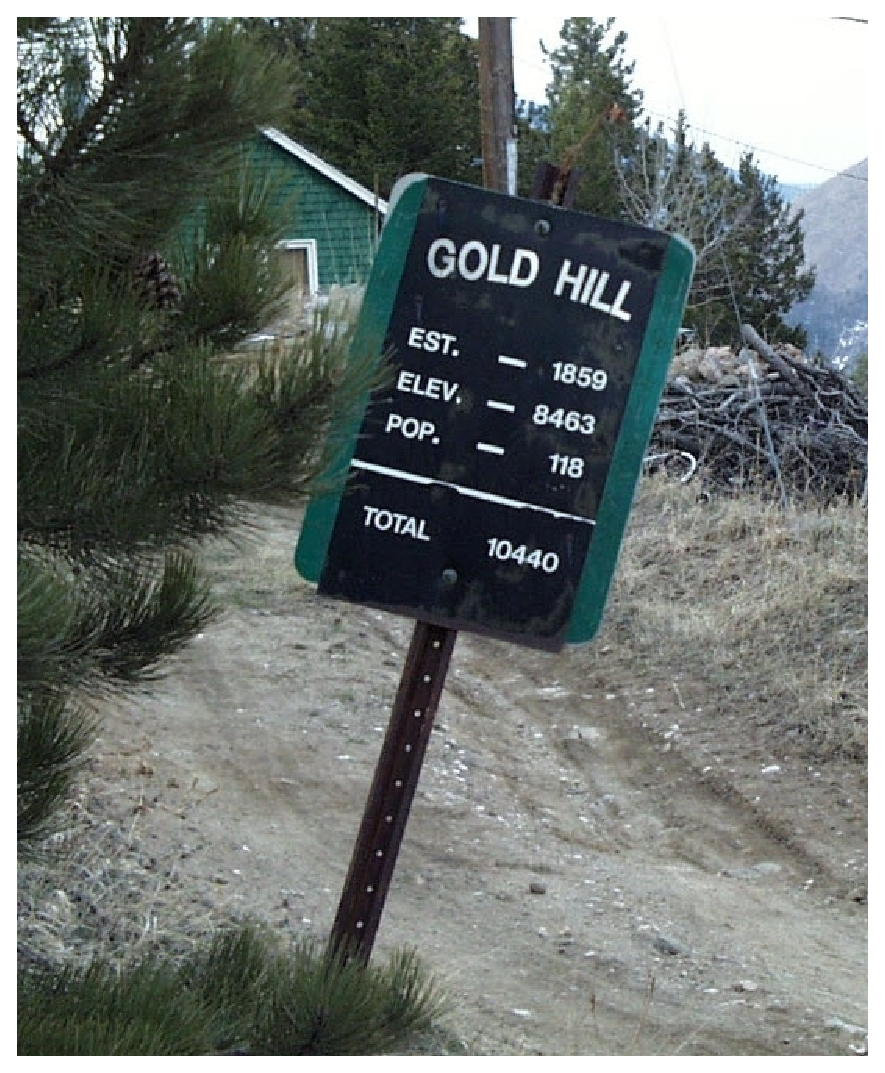
\includegraphics[width=5cm]{type-error}
\par\end{centering}
\caption{A nonsensical calculation arises when mixing incompatible data types.}
\label{nonsense-math}
\end{figure}

The power of the basic principles of mathematics extends over all
epochs and all cultures; they are the same in Rio de Janeiro, in Kuala-Lumpur,
and even in Pyongyang (see Fig.\ \ref{code-without-bugs}).

\section{Functional programming is math}

The functional programming paradigm is based on similar principles:
values are immutable, data processing is coded through formula-like
expressions, and each type of data is required to match correctly
during the computations. A flexible system of data types helps programmers
automatically prevent many kind of coding errors. In addition, modern
programming languages such as Scala and Haskell have a set of features
adapted to building powerful abstractions and domain-specific languages.
This power of abstraction is not accidental. Since mathematics is
the ultimate art of building abstractions, math-based functional programming
languages capitalize on the advantage of several millennia of mathematical
experience.

A prominent example of how mathematics informs the design of programming
languages is the connection between \href{https://en.wikipedia.org/wiki/Intuitionistic_logic}{constructive logic}
and the programming language's type system, called the \href{https://en.wikipedia.org/wiki/Curry\%E2\%80\%93Howard_correspondence}{Curry-Howard (CH) correspondence}.
The main idea of the CH correspondence\index{Curry-Howard correspondence}
is to think of programs as mathematical formulas that compute a value
of a certain type $A$. The CH correspondence is between programs
and logical propositions. To any program that computes a value of
type $A$, there corresponds a proposition stating that ``a value
of type $A$ can be computed''.

This may sound rather theoretical so far. To see the real value of
the CH correspondence, recall that formal logic has operations ``\textbf{\emph{and}}'',
``\textbf{\emph{or}}'', and ``\textbf{\emph{implies}}''. For any
two propositions $A$, $B$, we can construct the propositions ``$A$
\textbf{\emph{and}} $B$'', ``$A$ \textbf{\emph{or}} $B$'', ``$A$
\textbf{\emph{implies}} $B$''. These three logical operations are
foundational; without one of them, the logic is \emph{incomplete}
(you cannot derive some theorems).

A programming language \textbf{obeys the CH correspondence}\index{Curry-Howard correspondence}
to the logic if for any two types $A$, $B$, the language also contains
composite types corresponding to the logical formulas ``$A$ \textbf{\emph{or}}
$B$'', ``$A$ \textbf{\emph{and}} $B$'', ``$A$ \textbf{\emph{implies}}
$B$''. In Scala, these composite types are \texttt{Either{[}A,B{]}},
the tuple \texttt{(A,B)}, and the function type, \texttt{A$\Rightarrow$B}.
All modern functional languages such as OCaml, Haskell, Scala, F\#,
Swift, Elm, and PureScript support these three type constructions
and thus are faithful to the CH correspondence. Having a \emph{complete}
logic in a language's type system enables \href{https://fsharpforfunandprofit.com/ddd/}{declarative domain-driven code design}.

It is interesting to note that most older programming languages (C/C++,
Java, JavaScript, Python) do not support some of these composite types.
In other words, these programming languages have type systems based
on an incomplete logic. As a result, users of these languages have
to implement burdensome workarounds that make for error-prone code.
Failure to follow mathematical principles has real costs.

\begin{figure}
\begin{centering}
\includegraphics[width=0.75\textwidth]{no-bugs}
\par\end{centering}
\caption{The Pyongyang method of error-free programming.}
\label{code-without-bugs}
\end{figure}


\section{The power of abstraction}

Data engineering at scale poses problems of such complexity that many
software companies adopt functional programming languages as their
main implementation tool. Netflix, LinkedIn, Twitter started using
Scala early on and were able to reap the benefits of the powerful
abstractions Scala affords, such as asynchronous streams and parallelized
functional collections. In this way, Scala enabled these businesses
to engineer and scale up their massively concurrent computations.
What exactly makes Scala suitable for big data processing?

The only way to manage massively concurrent code is to use sufficiently
high-level abstractions that make application code declarative. The
two most important such abstractions are the ``resilient distributed
dataset'' (RDD) of Apache Spark and the ``reactive stream'' used
in systems such as Kafka, Apache Storm, Akka Streams, and Apache Flink.
While these abstractions are certainly implementable in Java or Python,
true declarative and type-safe usage is possible only in a programming
language with a sufficiently sophisticated functional type system.
Among the currently available mature functional languages, only Scala
and Haskell would be technically adequate for that task, due to their
support for typeclasses and higher-order generic collections.

It remains to see why Scala became the \emph{lingua franca} of big
data and not, say, Haskell.

\section{Scala is Java on math }

The recently invented general-purpose functional programming languages
can be grouped into ``industrial'' (F\#, Scala, Swift) and ``academic''
(OCaml, Haskell).

The ``academic'' languages are clean-room implementations of well-researched
mathematical principles of programming language design (the CH correspondence
being one such principle). These languages are unencumbered by requirements
of compatibility with any existing platform or libraries. Because
of this, the ``academic'' languages are perfect playgrounds for
taking various mathematical ideas to their logical conclusion. At
the same time, software practitioners struggle to adopt these languages
due to a steep learning curve, a lack of enterprise-grade libraries
and tool support, and immature package management.

The languages from the ``industrial'' group are based on existing
and mature software ecosystems: F\# on .NET, Scala on JVM, and Swift
on Apple's MacOS/iOS platform. One of the important design requirements
for these languages is 100\% binary compatibility with their ``parent''
platforms and languages (F\# with C\#, Scala with Java, and Swift
with Objective-C). Because of this, developers can immediately take
advantage of the existing tooling, package management, and industry-strength
libraries, while slowly ramping up the idiomatic usage of new language
features. However, the same compatibility requirements necessitated
certain limitations in the languages, making their design less than
fully satisfactory from the functional programming viewpoint.

It is now easy to see why the adoption rate of the ``industrial''
group of languages is \href{https://www.tiobe.com/tiobe-index/}{much higher}
than that of the ``academic'' languages. The transition to the functional
paradigm is also made smoother for software developers because F\#,
Scala, and Swift seamlessly support the familiar object-oriented programming
paradigm. At the same time, these new languages still have logically
complete type systems, which gives developers an important benefit
of type-safe domain modeling.

Nevertheless, the type systems of these languages are not equally
powerful. For instance, F\# and Swift are similar to OCaml in many
ways but omit OCaml's parameterized modules and some other features.
Of all mentioned languages, only Scala and Haskell directly support
typeclasses and higher-order generics, which are necessary for expressing
abstractions such as automatically parallelized data sets or asynchronous
data streams.

To see the impact of these advanced features of Scala and Haskell,
consider LINQ, a domain-specific language for database queries on
.NET, implemented in C\# and F\# through a special built-in syntax
supported by Microsoft's compilers. Analogous functionality is provided
in Scala as a \emph{library}, without need to modify the Scala compiler,
by several open-source projects such as Slick, Squeryl, or Quill.
Similar libraries exist for Haskell \textendash{} but are impossible
to implement in languages with less powerful type systems.

\section{Conclusion}

The decisive advantages of Scala over other contenders (such as OCaml,
Haskell, F\#, or Swift) are
\begin{enumerate}
\item functional collections in the standard library;
\item a highly sophisticated type system, with support for typeclasses and
higher-order generics; 
\item seamless compatibility with a mature software ecosystem (JVM). 
\end{enumerate}
Based on this assessment, we may be confident in Scala's great future
as a main implementation language for big data engineering. 

\chapter{``Applied functional type theory'': A proposal}

What exactly is the extent of ``theory'' that a practicing functional
programmer should know in order to be effective at writing code in
the functional paradigm? In my view, this question is not yet resolved.
In this book, I present a coherent body of theoretical knowledge that
I believe fits the description of ``practicable functional programming
theory''. This body of knowledge is, or should be, understood as
a branch of computer science, and I propose to call it\textbf{ \index{applied functional type theory}applied
functional type theory} (AFTT). This is the area of theoretical computer
science that should serve the needs of functional programmers working
as software engineers.

It is for these practitioners (I am one myself), rather than for academic
researchers, that I set out to examine the functional programming
inventions over the last 30 years, \textendash{} such as the \href{https://wiki.haskell.org/Research_papers/Functional_pearls}{\textquotedblleft functional pearls\textquotedblright{} papers}
\textendash{} and to determine the scope of theoretical material that
has demonstrated its pragmatic usefulness and thus belongs to AFTT,
as opposed to material that is purely academic and may be tentatively
omitted. This book is a first step towards formulating AFTT.

In this book, I show code in Scala because I am familiar with that
language. However, most of this material will work equally well in
Haskell, OCaml, and other FP languages. This is so because the science
of functional programming, which I call AFTT, is not a set of tricks
specific to Scala or Haskell. An advanced user of any other functional
programming language will have to face the same questions and struggle
with the same practical issues.

\section{AFTT is not covered by computer science curricula}

Traditional courses of theoretical computer science (algorithms and
data structures, complexity theory, distributed systems, databases,
network systems, compilers, operating systems) are largely not relevant
to AFTT.

Here is an example: To an academic computer scientist, the ``science
behind Haskell'' is the theory of lambda-calculus, the type-theoretic
``System $F\omega$'', and formal semantics. These theories guided
the design of the Haskell language and define rigorously what a Haskell
program ``means'' in a mathematical sense. Academic computer science
courses teach these theories, although typically only at the graduate
level. 

However, a practicing Haskell or Scala programmer is not concerned
with designing Haskell or Scala, or with proving any theoretical properties
of those languages. A practicing programmer is mainly concerned with
\emph{using} a chosen programming language to \emph{write code}. 

Neither the theory of lambda-calculus, nor proofs of type-theoretical
properties of ``System $F\omega$'', nor theories of formal semantics
will actually help a programmer to write code. So all these theories
are not within the scope of AFTT. Functional programming does not
require graduate-level theoretical studies.

As an example of theoretical material that \emph{is} within the scope
of AFTT, consider the equational laws imposed on applicative functors
(see Chapter~\ref{chap:8-Applicative-functors,-contrafunc}).\index{applicative functors} 

It is essential for a practicing functional programmer to be able
to recognize and use applicative functors. An applicative functor
is a data structure specifying declaratively a set of operations that
run independently of each other. Programs can then easily combine
these operations, for example, in order to execute them in parallel,
or to refactor the program for better maintainability.

To use this functionality, the programmer must begin by checking whether
a given data structure satisfies the laws of applicative functors.
In a given application, a data structure may be dictated in part by
the business logic rather than by a programmer's choice. The programmer
first writes down the type of that data structure and the code implementing
the required methods, and then checks that the laws hold. The data
structure may need to be adjusted in order to fit the definition of
an applicative functor or its laws.

This work is done using pen and paper, in a mathematical notation.
Once the applicative laws are verified, the programmer proceeds to
write code using that data structure.

Because of the mathematical proofs, it is assured that the data structure
satisfies the known properties of applicative functors, no matter
how the rest of the program is written. So, for example, it is assured
that the relevant effects can be automatically parallelized and will
still work correctly. In this way, AFTT directly guides the programmer
and helps to write correct code.

Applicative functors were discovered by practitioners who were using
Haskell for writing code, in applications such as parser combinators,
compilers, and domain-specific languages for parallel computations.
However, applicative functors are not a feature of Haskell: they are
the same in Scala, OCaml, or any other functional programming language.
And yet, no standard computer science textbook defines applicative
functors, motivates their laws, explores their structure on basic
examples, or shows data structures that are \emph{not} applicative
functors and explains why. (Books on category theory and type theory
also do not mention applicative functors.)\index{applicative functors}

\section{AFTT is not category theory, type theory, or formal logic}

So far it appears that AFTT includes a selection of certain areas
of category theory, formal logic, and type theory. However, software
engineers would not derive much benefit from following traditional
academic courses in these subjects, because their presentation is
too abstract and at the same time lacks specific results necessary
for practical programming. In other words, the traditional academic
courses answer questions that academic computer scientists have, not
questions that software engineers have.

There exist several books intended as presentations of category theory
``for computer scientists'' or ``for programmers''. However, these
books do not explain certain concepts relevant to programming, such
as applicative or traversable functors. Instead, these books contain
purely theoretical topics such as limits, adjunctions, or toposes,
\textendash{} concepts that have no applications in practical functional
programming today.

Typical questions in academic books are: ``Is $X$ an introduction
rule or an elimination rule'' and ``Does the property $Y$ hold
in non-small categories, or only in the category of sets''. Typical
questions a Scala programmer might have are: ``Can we compute a value
of type \lstinline!Either[Z, R => A]! from a value of type \lstinline!R => Either[Z, A]!''
and ``Is the type constructor \lstinline!F[A] = Option[(A, A, A)]!
a monad or only an applicative functor''. The proper scope of AFTT
includes answering the last two questions, but \emph{not} the first
two.

A software engineer hoping to understand the foundations of functional
programming will not find the concepts of filterable, applicative,
or traversable functors in any books on category theory, including
books intended for programmers. And yet, these concepts are necessary
to obtain a mathematically correct implementation of such foundationally
important operations as \lstinline!filter!, \lstinline!zip!, and
\lstinline!traverse! \textendash{} operations that functional programmers
often use in their code.

To compensate for the lack of AFTT textbooks, programmers have written
many online tutorials for each other, trying to explain the theoretical
concepts necessary for practical work. There are the infamous ``monad
tutorials'', but also tutorials about applicative functors, traversable
functors, free monads, and so on. These tutorials tend to be hands-on
(``run this code now and see what happens'') and narrow in scope,
limited to one or two specific questions and specific applications.
Such tutorials usually do not present sufficient mathematical insights
to help programmers develop the necessary mathematical intuition.

For example, ``free monads'' became popular in the Scala community
around 2015. Many talks about free monads were presented at Scala
engineering conferences, each giving their own slightly different
implementation but never formulating rigorously the required properties
for a piece of code to be a valid implementation of the free monad.

Without knowledge of mathematical principles behind free monads, a
programmer cannot make sure that a given implementation is correct.
However, books on category theory present free monads in a way that
is unsuitable for programming applications: a free monad is just an
adjoint functor to a forgetful functor into the category of sets.\footnote{``What's your problem?'' as the joke would go.}
This definition is too abstract and, for instance, cannot be used
to check whether a given implementation of the free monad in Scala
is correct.

Perhaps the best selection of AFTT tutorial material can be found
in the \href{https://en.wikibooks.org/wiki/Haskell}{Haskell Wikibooks}.
However, those tutorials are incomplete and limited to explaining
the use of Haskell. Many of them are suitable neither as a first introduction
nor as a reference on AFTT. Also, the Haskell Wikibooks tutorials
rarely show any proofs or derivations of equational laws.

Apart from referring to some notions from category theory, AFTT also
uses some concepts from type theory and formal logic. However, existing
textbooks on type theory and formal logic focus on domain theory and
proof theory \textendash{} which is a lot of information that practicing
programmers will have difficulty assimilating and yet will have no
chance of ever applying in their daily work. At the same time, these
books never mention practical techniques used in many functional programming
libraries today, such as quantified types, types parameterized by
type constructors, or partial type-level functions (known as ``typeclasses'').

Type theory and formal logic can, in principle, help the programmer
with certain practical tasks, such as:
\begin{itemize}
\item deciding whether two data structures are equivalent as types, and
implementing the isomorphism transformation; for example, the Scala
type \lstinline!(A, Either[B, C])! is equivalent to \lstinline!Either[(A, B), (A, C)]! 
\item detecting whether a definition of a recursive type is ``reasonable'',
i.e.~does not lead to a useless infinite recursion; an example of
a useless recursive type definition in Scala is \lstinline!case class Bad(x: Bad)! 
\item deriving an implementation of a function from its type signature and
required laws; for example, deriving the \lstinline!flatMap! method
for the \lstinline!Reader! monad from the type signature 
\begin{lstlisting}
def flatMap[Z, A, B](r: Z => A)(f: A => Z => B): Z => B
\end{lstlisting}
 and verifying that the monad laws hold
\item deciding whether a generic pure function with a given signature can
be implemented; for example, \lstinline!def f[A, B]: (A => B) => A!
cannot be implemented but \lstinline!def g[A, B]: A => (B => A)!
can be implemented 
\end{itemize}
I mention these practical tasks as examples because they are actual
real-world-coding applications of domain theory and the Curry-Howard
correspondence theory. However, existing books on type theory and
logic do not give practical recipes for resolving these questions.

On the other hand, books such as \href{https://underscore.io/books/scala-with-cats/}{\textquotedblleft Scala with Cats\textquotedblright}
and \href{https://alvinalexander.com/scala/functional-programming-simplified-book}{\textquotedblleft Functional programming, simplified\textquotedblright}
are focused on explaining the practical aspects of programming and
do not adequately treat the equational laws that the mathematical
structures require (such as the laws for applicative or monadic functors).

The only existing Scala-based AFTT textbook aiming at the proper scope
is the \href{https://www.manning.com/books/functional-programming-in-scala}{Bjarnason-Chiusano book},
which balances practical considerations with theoretical developments
such as equational laws. This book is written at about the same level
but goes deeper into the mathematical foundations and at the same
time gives a wider range of examples.

This book is an attempt to delineate the proper scope of AFTT and
to develop a rigorous yet clear and approachable presentation of the
chosen material. 
